\documentclass[tikz]{standalone}

\usetikzlibrary{matrix, positioning}

\usepackage{xcolor}
\colorlet{myred}{red!80!black}
\colorlet{myblue}{blue!80!black}
\colorlet{mybluee}{myblue!80!black}
\colorlet{mygreen}{green!60!black}
\colorlet{mydarkred}{red!30!black}
\colorlet{mydarkblue}{blue!40!black}
\colorlet{mydarkgreen}{green!30!black}

\begin{document}
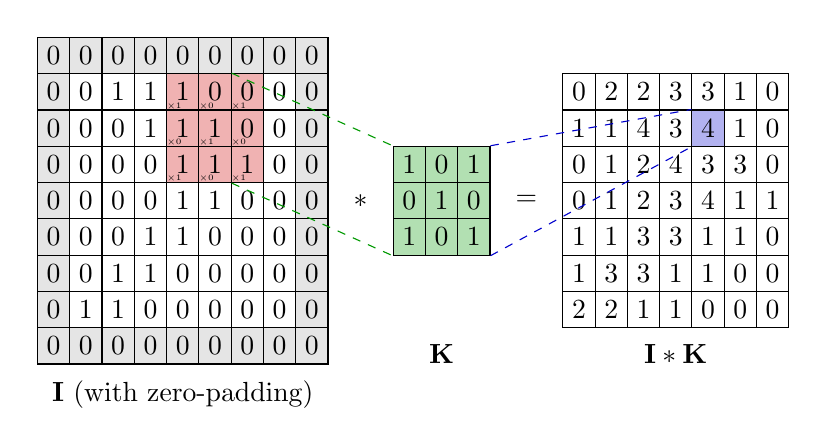
\begin{tikzpicture}[
    2d-arr/.style={matrix of nodes, row sep=-\pgflinewidth, column sep=-\pgflinewidth, nodes={draw}}
  ]
  \matrix (mtr) [2d-arr] {
  |[fill=gray!20]| 0 & |[fill=gray!20]| 0 & |[fill=gray!20]| 0 & |[fill=gray!20]| 0 & |[fill=gray!20]| 0 & |[fill=gray!20]| 0 & |[fill=gray!20]| 0 & |[fill=gray!20]| 0 & |[fill=gray!20]| 0 \\
  |[fill=gray!20]| 0 & 0 & 1 & 1 & |[fill=myred!30]| 1 & |[fill=myred!30]| 0 & |[fill=myred!30]| 0 & 0 & |[fill=gray!20]| 0 \\
  |[fill=gray!20]| 0 & 0 & 0 & 1 & |[fill=myred!30]| 1 & |[fill=myred!30]| 1 & |[fill=myred!30]| 0 & 0 & |[fill=gray!20]| 0 \\
  |[fill=gray!20]| 0 & 0 & 0 & 0 & |[fill=myred!30]| 1 & |[fill=myred!30]| 1 & |[fill=myred!30]| 1 & 0 & |[fill=gray!20]| 0 \\
  |[fill=gray!20]| 0 & 0 & 0 & 0 & 1 & 1 & 0 & 0 & |[fill=gray!20]| 0 \\
  |[fill=gray!20]| 0 & 0 & 0 & 1 & 1 & 0 & 0 & 0 & |[fill=gray!20]| 0 \\
  |[fill=gray!20]| 0 & 0 & 1 & 1 & 0 & 0 & 0 & 0 & |[fill=gray!20]| 0 \\
  |[fill=gray!20]| 0 & 1 & 1 & 0 & 0 & 0 & 0 & 0 & |[fill=gray!20]| 0 \\
  |[fill=gray!20]| 0 & |[fill=gray!20]| 0 & |[fill=gray!20]| 0 & |[fill=gray!20]| 0 & |[fill=gray!20]| 0 & |[fill=gray!20]| 0 & |[fill=gray!20]| 0 & |[fill=gray!20]| 0 & |[fill=gray!20]| 0 \\
  };
  \node[below=of mtr-7-5] {$\mathbf I$ (with zero-padding)};
  \node[right=0.2em of mtr] (str) {$*$};
  \matrix (K) [2d-arr, right=0.2em of str, nodes={draw, fill=mygreen!30}] {
    1 & 0 & 1 \\
    0 & 1 & 0 \\
    1 & 0 & 1 \\
  };
  \node[below=of K-3-2] {$\mathbf K$};
  \node[right=0.2em of K] (eq) {$=$};
  \matrix (ret) [2d-arr, right=0.2em of eq] {
  0 & 2 & 2 & 3 & 3 & 1 & 0 \\
  1 & 1 & 4 & 3 & |[fill=blue!80!black!30]| 4 & 1 & 0 \\
  0 & 1 & 2 & 4 & 3 & 3 & 0 \\
  0 & 1 & 2 & 3 & 4 & 1 & 1 \\
  1 & 1 & 3 & 3 & 1 & 1 & 0 \\
  1 & 3 & 3 & 1 & 1 & 0 & 0 \\
  2 & 2 & 1 & 1 & 0 & 0 & 0 \\
  };
  \node[below=of ret-5-4] {$\mathbf{I * K}$};
  \draw[dashed, mygreen] (mtr-2-6.north east) -- (K-1-1.north west);
  \draw[dashed, mygreen] (mtr-4-6.south east) -- (K-3-1.south west);
  \draw[dashed, blue!80!black] (K-1-3.north east) -- (ret-2-5.north west);
  \draw[dashed, blue!80!black] (K-3-3.south east) -- (ret-2-5.south west);
  \foreach \i in {2,3,4} {
      \foreach \j in {5,6,7} {
          \node[font=\tiny, scale=0.6, shift={(-1.2ex,-2ex)}] at (mtr-\i-\j) {$\times \pgfmathparse{int(mod(\i+\j,2))}\pgfmathresult$};
        }
    }
\end{tikzpicture}
\end{document}